\section{Inverted Indices}

\subsection{Implementation}
Based on the prototype for the project we implemented two inverted indexes. The InvertedIndexHashMap and InvertedIndexTreeMap are two subclasses of the superclass InvertedIndex which in turn implements the Index interface. The inverted index is a clever implementation of the SimpleIndex class trying to overcome the problems given by this naive implementation which for every query given looks through every website in the database. The purpose of an inverted index is to preemptively create an index of websites to word when the program is build, rather than performing the task at every query. In this scenario when a user makes a query the search will be performed on a Map object which maps words contained in the websites, to the website objects. In this way we increase the time needed for building the application, but we decrease the time needed for every single query. This results in an overall improvement of the performance.

The two subclasses have only one difference, they instantiate two different dynamic types of the map object. A Map is an interface which once implemented by a class will map a key to a value. The key needs to be unique but the value can be repeated.
The InvertedIndexHashMap inherits all the methods and variables from the abstract superclass InvertedIndex and instantiate a HashMap. The HashMap is an implementation of the Map interface, it maps a data value (in this case a Collection<Website>) to a specific key (in this case a string which represents one word present in a specific Website). The HashMap does not follow any index and the order of the objects contained can change over time.
On the other hand we have the InvertedIndexTreeMap, which instantiate a TreeMap dynamic type for the map variable and inherits all the methods and variables from the abstract superclass InvertedIndex. The TreeMap follows the same behaviour as the HashMap with only one important difference, the TreeMap has an ordered index of its mappings. The TreeMap is sorted following the natural order of the keys or according to a provided Comparator. In our case this means that the String key will be sorted alphabetically.

As previously mentioned, these two classes extend the superclass InvertedIndex which is an abstract class, this means that is not possible to instantiate an InvertedIndex object directly. This structure allows us to write the code in a more structured way, avoiding duplicate code and leading to easy extensibility of the application. Hence, we implement all the common behaviour of an index into the InvertedIndex superclass and then we implement the details into the specific subclasses.

When we create an object using a subclass as dynamic type, the constructor of the subclass will initialize the map object respectively as a HashMap or a TreeMap. Then when a method is called on the object, the compiler will perform a method-lookup, which means that it will look for the method in the subclass. But in this case it will find only the constructor, then it will look into the superclass that contain the build method and the lookup method. These two methods will perform their operations on the map object which was initialized into the sub-class constructor, so we use a TreeMap or a HashMap depending on the dynamic type declared at the object creation.


\begin{figure}[t]
	\centering
	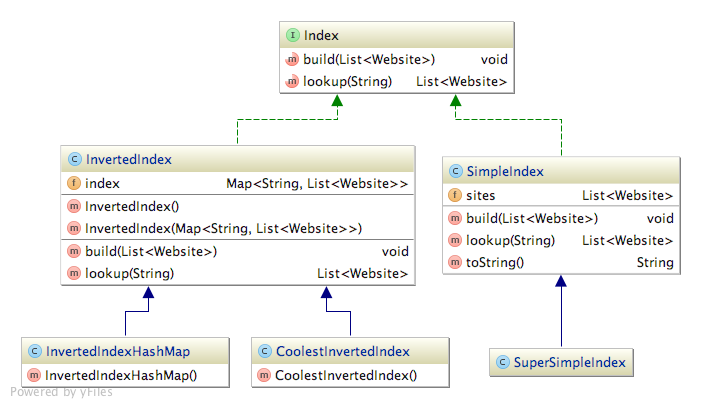
\includegraphics[width=\textwidth]{graphics/diagram-index.png}
	\caption{UML Diagram for the Software Architecture of Index data structures.}
	\label{fig:index:uml}
\end{figure}



\subsection{Benchmarking}
The different index implementations of the were to be benchmarked and compared. 
The benchmarking process would look up a list of 20 different queries, on a given database file with a given index. The expected findings in terms of performance were that the \code{TreeMap} implementation would faster than the \code{HashMap} implementation on larger data file sizes. This expectation was due to \code{TreeMap} having a logarithmic growth in time cost of the \code{.get} method proportionate to map size, compared to the constant growth in time cost for the \code{HashMap}. \\
The efficiency of the two indices was then expected to intersect at some map size, with \code{HashMap} being the most efficient up until the intersection size and then the \code{TreeMap} would be the most efficient of sizes bigger than that. \\
The benchmark was applied on all the handed out file sizes and for all the available index implementations. The results of the benchmarking can be found in Table \ref{tab:benchmark:indices}.

\paragraph{Analysis and discussion:}
The results of the benchmarking did not align completely with our expectations. As can be seen from the results, the \code{InvertedIndexTreeMap} did not manage to outperform \code{InvertedIndexHashMap}. This was probably due to the data files not having a sufficient size for \code{TreeMap} to overshadow the \code{HashMap}. The performance for the two inverted indices were very similar, with the relative difference deteriorating as the data file sizes increase. Judging from the development in the differences it would take a significantly bigger data size for the \code{TreeMap} to be the better option. Since we do expect to end up using a much bigger data file, and the negligible difference between the two in general we decided to keep the \code{TreeMap} implementation in our code for now.

\begin{table}[t]
\centering
\begin{tabular}{llrr} \toprule
	Index					& File size & Avg LUT 	& $\pm$ Error \\ \midrule
	SimpleIndex				& tiny		& 22.92  	&	 0.76 \\ 
						 	& small		& 10832.42 	&	 2088.43 \\
							& medium 	& 283513.44 & 	 7717.45 \\ \hline
	InvertedIndexTreeMap	& tiny 		& 5.44 		& 	 0.29 \\
							& small 	& 9.28 		& 	 0.20  \\
							& medium 	& 135.26 	& 	 2.57 \\ \hline
	InvertedIndexHashMap	& tiny		& 4.68 		& 	 0.15 \\
							& small		& 8.16 		& 	 0.30 \\
							& medium 	& 120.40 	& 	 4.36 \\ \bottomrule
\end{tabular}
	\caption{Running times for different index implementations.}	
\label{tab:benchmark:indices}
\end{table} 	
